%%% Preamble starts here.
\documentclass{amsart}
%for the heading
\usepackage{fancyhdr, enumerate}
%for the picture. 
\usepackage{tikz, calc}
%adjust the page width
\usepackage[margin=1in]{geometry}

%% The next line says how the "vertex" style of nodes should look: drawn as small circles.
\tikzstyle{vertex}=[circle, draw, inner sep=0pt, minimum size=6pt,fill=white]
%%
%% Next, we make a \vertex command as a shorthand in place of \node[vertex} to get that style.
\newcommand{\vertex}{\node[vertex]}

\linespread{1.1}


%special commands for number sets
\def\RR{{\mathbb R}}
\def\NN{{\mathbb N}}
\def\ZZ{{\mathbb Z}}
\def\QQ{{\mathbb Q}}
\def\CC{{\mathbb C}}

% header
\lhead{\sc  MATH 490 Senior Seminar}
\chead{\sc Midterm} 
\rhead{Monday 2 March 2020}
\cfoot{}
\pagestyle{fancy}

%%%% Main document starts here.

\begin{document}
\thispagestyle{fancy}

\vskip 2cm
{\fontsize{18}{22}{Rules:}}

You have 60 minutes to complete the exam.  

Unless otherwise stated, full credit will only be given for formal proofs.

Partial credit will be awarded, but you must show your work.

No calculators, books, notes, or other aids are permitted.  

If you need extra space, you can use the back sides of the pages.  (Clearly label any work you want graded.)

Turn off anything that might go beep during the exam.

Good luck!

\vskip 1cm
\def\emptybox{\hbox to 2em{\vrule height 16pt depth 8pt width 0pt\hfil}}
\def\tline{\noalign{\hrule}}
\centerline{\vbox{\offinterlineskip
{
\bf\sf\fontsize{18pt}{22pt}\selectfont
\hrule
\halign{
\vrule#&\strut\quad\hfil#\hfil\quad&\vrule#&\quad\hfil#\hfil\quad
&\vrule#&\quad\hfil#\hfil\quad&\vrule#\cr
height 3pt&\omit&&\omit&&\omit&\cr
&Problem&&Possible&&Score&\cr\tline
height 3pt&\omit&&\omit&&\omit&\cr
&1&& 10 &&\emptybox&\cr\tline
&2&&12 &&\emptybox&\cr\tline
&3&& 12 &&\emptybox&\cr\tline
&4&& 10 &&\emptybox&\cr\tline
&5&&16 &&\emptybox&\cr\tline
&6&& 10 &&\emptybox&\cr\tline
&Extra Credit&&3&&\emptybox&\cr\tline
&Total&&70 &&\emptybox&\cr
}\hrule}}}

\vfill
{\Large{\textbf{NAME:}}} 
\vfill

\newpage
 
\begin{enumerate}
\item (10 points) Prove \textbf{Corollary 1.3.4:}\\ 
In a graph $G$, the average degree of a vertex is $\displaystyle{\frac{2 e(G)}{n(G)}}$ and hence $\displaystyle{\delta(G) \leq \frac{2 e(G)}{n(G)} \leq \Delta(G).}$\\
(Make sure to address both parts of this statement.)

\newpage
\item (12 points) \begin{enumerate}
	\item Prove that if $G$ is a graph with at least 2 vertices, deleting a vertex of degree $\Delta(G)$ \textbf{cannot} increase the average degree of $G.$
	\vfill
	\item Prove that if $G$ is a graph with at least 2 vertices, deleting a vertex of degree $\delta(G)$ \textbf{can} decrease the average degree of $G.$
	\vspace{3in}
	\end{enumerate}
\newpage
\item (10 points) \textbf{Sketch} the proof of the theorem below. Your sketch should include the proof technique, underlying logic and any lemmas or earlier results on which the argument depends. The basic structure should be present, though some details may be omitted.\\

\begin{quote} \textbf{Theorem 1.2.26} A graph is Eulerian if and only if has at most one nontrivial component and its vertices all have even degree.\end{quote}
\newpage
\item (10 points) Prove \textbf{Corollary 3.1.13:} For every $k > 0,$ every $k$-regular bipartite graph has a perfect matching. \\
\newpage
\item (16 points) The graph $G$ is below. It is copied below each questions in case you would like to draw your answer on a copy of the graph. Examples or short explanations are sufficient. No proofs required here.\\

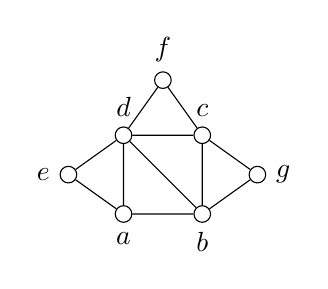
\begin{tikzpicture}
\vertex (a) at (0,0)[label=below:$a$]{};
\vertex (b) at (1,0)[label=below:$b$]{};
\vertex (c) at (1,1)[label=above:$c$]{};
\vertex (d) at (0,1)[label=above:$d$]{};
\vertex (e) at (-0.7,0.5)[label=left:$e$]{};
\vertex (f) at (0.5,1.7)[label=above:$f$]{};
\vertex (g) at (1.7,0.5)[label=right:$g$]{};
\draw (a)--(b)--(c)--(d)--(a)--(e)--(d)--(f)--(c)--(g)--(b)--(d);
\end{tikzpicture}

	\begin{enumerate}
	\item Find a path in $G$ that is maximal but not maximum or explain  that one does not exist.\\
	
	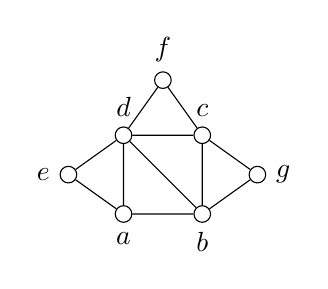
\begin{tikzpicture}
\vertex (a) at (0,0)[label=below:$a$]{};
\vertex (b) at (1,0)[label=below:$b$]{};
\vertex (c) at (1,1)[label=above:$c$]{};
\vertex (d) at (0,1)[label=above:$d$]{};
\vertex (e) at (-0.7,0.5)[label=left:$e$]{};
\vertex (f) at (0.5,1.7)[label=above:$f$]{};
\vertex (g) at (1.7,0.5)[label=right:$g$]{};
\draw (a)--(b)--(c)--(d)--(a)--(e)--(d)--(f)--(c)--(g)--(b)--(d);
\end{tikzpicture}
	\item A matching in $G$ that is maximal but not maximum or explain  that one does not exist.\\
	
	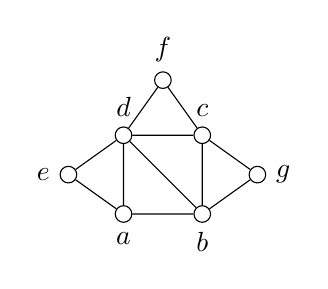
\begin{tikzpicture}
\vertex (a) at (0,0)[label=below:$a$]{};
\vertex (b) at (1,0)[label=below:$b$]{};
\vertex (c) at (1,1)[label=above:$c$]{};
\vertex (d) at (0,1)[label=above:$d$]{};
\vertex (e) at (-0.7,0.5)[label=left:$e$]{};
\vertex (f) at (0.5,1.7)[label=above:$f$]{};
\vertex (g) at (1.7,0.5)[label=right:$g$]{};
\draw (a)--(b)--(c)--(d)--(a)--(e)--(d)--(f)--(c)--(g)--(b)--(d);
\end{tikzpicture}
	\item Find a circuit that is not a cycle or explain why one does not exist.\\
	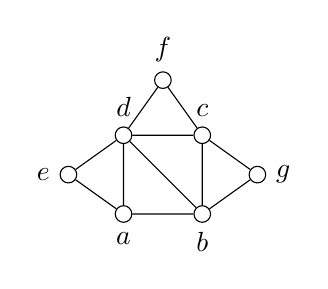
\begin{tikzpicture}
\vertex (a) at (0,0)[label=below:$a$]{};
\vertex (b) at (1,0)[label=below:$b$]{};
\vertex (c) at (1,1)[label=above:$c$]{};
\vertex (d) at (0,1)[label=above:$d$]{};
\vertex (e) at (-0.7,0.5)[label=left:$e$]{};
\vertex (f) at (0.5,1.7)[label=above:$f$]{};
\vertex (g) at (1.7,0.5)[label=right:$g$]{};
\draw (a)--(b)--(c)--(d)--(a)--(e)--(d)--(f)--(c)--(g)--(b)--(d);
\end{tikzpicture}
	\item Find a bipartite subgraph of $G$ containing at least half of the edges.\\
	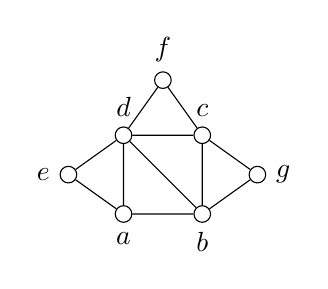
\begin{tikzpicture}
\vertex (a) at (0,0)[label=below:$a$]{};
\vertex (b) at (1,0)[label=below:$b$]{};
\vertex (c) at (1,1)[label=above:$c$]{};
\vertex (d) at (0,1)[label=above:$d$]{};
\vertex (e) at (-0.7,0.5)[label=left:$e$]{};
\vertex (f) at (0.5,1.7)[label=above:$f$]{};
\vertex (g) at (1.7,0.5)[label=right:$g$]{};
\draw (a)--(b)--(c)--(d)--(a)--(e)--(d)--(f)--(c)--(g)--(b)--(d);
\end{tikzpicture}
	\end{enumerate}
	\newpage
\item (10 points) Let $v$ be a cut vertex of a simple graph $G$. Prove that $\overline{G}-v$ is connected.
\end{enumerate}
\newpage
Extra Credit: (4 points) Prove that every simple graph with at least two vertices has two vertices of equal degree.
\end{document}



